\chapter{Metodología}

En esta sección se documentarán las metodologías empleadas para el seguimiento del desarrollo del proyecto. Al aplicar estas metodologías se ha conseguido una mayor eficiencia en la gestión del tiempo y de los recursos, así como una mayor calidad en la documentación y en el código fuente. Además, se explicarán las herramientas utilizadas para el control de versiones y el alojamiento del repositorio remoto del proyecto.

\section{Enfoque ágil}

El proyecto seguirá las prácticas y principios del enfoque ágil, que se fundamenta en los 17 principios delineados en \href{https://agilemanifesto.org/iso/es/manifesto.html}{el manifiesto ágil}. Ágil no es una metodología ni un marco de trabajo, sino una mentalidad que permite a las organizaciones ser más receptivas al cambio. Estos principios están diseñados para asegurar la satisfacción del cliente a través de la entrega temprana y continua de valor, con un fuerte enfoque en la excelencia técnica, el buen diseño, la planificación y la simplicidad.

Estos principios no son solo una referencia teórica, sino que se han aplicado con éxito en proyectos reales y actuales, de acuerdo con~\cite{berlas2024software}. Este informe presenta una revisión completa de la investigación publicada sobre las métricas de software en el desarrollo ágil y resalta su efectividad en diversos contextos, incluyendo pequeñas y medianas empresas.

\begin{itemize}
    \item \textbf{¿Se están usando enfoques ágiles?} El informe indica que los enfoques ágiles son ampliamente utilizados en la industria del software, permitiendo a los equipos de desarrollo trabajar iterativamente y responder rápidamente a las necesidades del cliente.
    \item \textbf{¿Esto verdaderamente funciona?} Según el informe, los enfoques ágiles han demostrado ser eficaces en diversos tipos de proyectos a cualquier escala proporcionando beneficios como la reducción del tiempo de comercialización, mayor satisfacción del cliente y disminución de los costos de desarrollo.
\end{itemize}

\section{Entrega y calidad continua}

Para asegurar la calidad del proyecto y la entrega continua, se han empleado una serie de herramientas y metodologías que se han integrado en el flujo de trabajo tanto local como remoto.

La documentación del proyecto es una de las partes más importantes (junto con el código) del trabajo de fin de grado si no la que más por lo que se ha de poner especial atención en que esta sea de calidad y cumpla con los requisitos establecidos por tutor y tribunal. Para dar cuenta de esto, la memoria se ha elaborado en \href{https://www.latex-project.org/}{\LaTeX{}} que es un sistema de composición tipográfica de alta calidad; este incluye funciones diseñadas para la producción de documentación técnica y científica además de estar disponible como software libre.

\subsection{Flujo de trabajo local}

Para complementar, comprobar y mejorar la calidad de la documentación se han usado una serie de herramientas que se han integrado en el flujo de trabajo local tanto con extensiones de (\href{https://code.visualstudio.com/}{\textit{Visual Studio Code}}) como con herramientas ejecutadas en la línea de comandos.

Más adelante se detallarán las herramientas utilizadas y el proceso de selección de las mismas.

\subsection{Flujo de trabajo remoto}

Estos flujos se realizan en \textit{GitHub} implementando uno específico para la memoria. Este flujo de trabajo se activa en cada \textit{push} y se encarga de ejecutar verificaciones gramaticales y ortográficas con \href{https://github.com/sylvainhalle/textidote}{\textit{TeXtidote}}~\ref{sec:textidote} de la cual se sube un informe y si pasa estas verificaciones de forma satisfactoria se sube la memoria compilada en formato PDF a modo de artefacto. Este flujo de trabajo remoto junto con el local garantizan la calidad de la documentación.

Ese artefacto generado tras acabar cada \textit{milestone} o hito podría ser perfectamente entregable a un cliente final a modo de entrega continua para que vea el progreso del proyecto. A mayores, hacemos referencia al tercer principio del \href{https://agilemanifesto.org/iso/es/principles.html}{manifiesto ágil} que dice: \textit{``Entregar software funcional frecuentemente, entre dos semanas y dos meses, con preferencia al periodo de tiempo más corto''}. Además, los flujos de trabajo remotos (en \textit{GitHub}) y locales promueven el noveno principio que hace referencia a la atención continua a la excelencia técnica y el buen diseño.

\section{Herramientas y metodologías utilizadas}

En esta sección se documentarán las metodologías empleadas para el seguimiento del desarrollo del proyecto. Al aplicar estas metodologías se ha conseguido una mayor eficiencia en la gestión del tiempo y de los recursos, así como una mayor calidad en la documentación y en el código fuente. Además, se explicarán las herramientas utilizadas para el control de versiones y el alojamiento del repositorio remoto del proyecto.

\subsection{\textit{Git y GitHub}: control de versiones y colaboración}

Para el control de versiones se ha empleado \textit{git} que es un sistema de control de versiones que permite llevar un control de los cambios en el código fuente.

Para la colaboración y hospedaje del código fuente se ha hecho en \textit{GitHub}, una plataforma que permite alojar proyectos de \textit{software} y colaborar en ellos. En \textit{GitHub} tenemos diferentes funcionalidades que han sido de ayuda para el desarrollo del proyecto.

\textbf{El repositorio del proyecto se puede encontrar en la siguiente dirección: \url{https://github.com/danigonzser/proyecto-tfg}.}

La transparencia y accesibilidad de GitHub facilitan la comunicación constante y la colaboración del equipo, apoyando los principios ágiles de la colaboración diaria entre desarrolladores y clientes, y de la construcción de proyectos en torno a individuos motivados.

En GitHub se integran diferentes herramientas que permiten llevar un control del desarrollo del proyecto. A continuación, se describen algunas de las funcionalidades más importantes.

\subsection{Extensión de \textit{Visual Studio Code}: \textit{LaTeX Workshop}}

LaTeX Workshop es una extensión para Visual Studio Code, cuyo objetivo es proporcionar funciones básicas para la composición tipográfica LaTeX con Visual Studio Code. Esta extensión proporciona una serie de características que facilitan la escritura de documentos en LaTeX como la previsualización en tiempo real, la compilación del documento, la visualización de errores y advertencias.

A mayores, esta extensión me ha permitido elegir la receta de compilación que se va a utilizar, la cual se ha configurado para que se compile la memoria junto con la bibliografía.

\begin{figure}[H]
    \caption{Captura de pantalla de \textit{Visual Studio Code} con la extensión \textit{LaTeX Workshop} activada.}
    \centering
    \vspace*{0.5cm}
    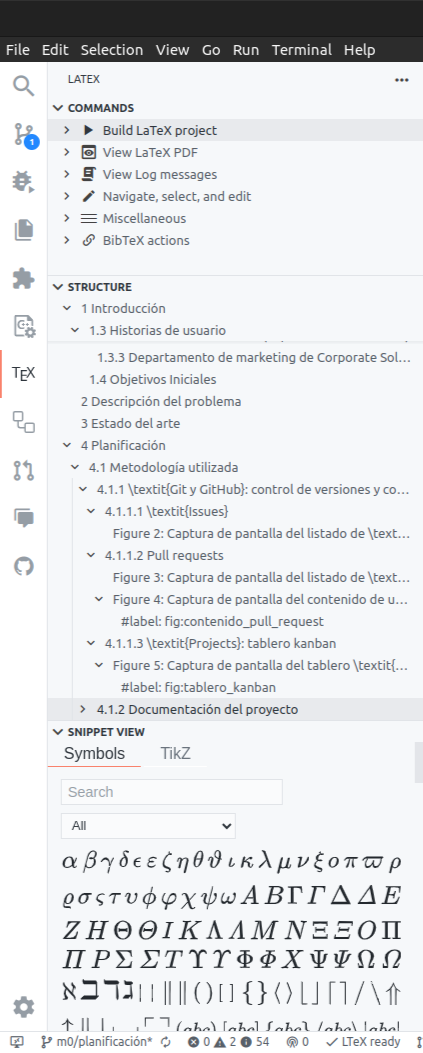
\includegraphics[scale=0.2]{figuras/latex_workshop_extension.png}\label{fig:latex_workshop_extension}
\end{figure}

\subsubsection{Extensión de \textit{Visual Studio Code}: \href{https://github.com/valentjn/vscode-ltex}{\textit{LTeX LanguageTool grammar/spell checking}}}

La extensión \( LT_E X \) permite comprobar la gramática y la ortografía de varios lenguajes de marcado en \textit{Visual Studio Code} mediante LanguageTool (véase~\ref{sec:languagetool}).

Esta extensión suele trabajar de forma offline teniendo una instancia local de \textit{LanguageTool}, pero en nuestro caso y para mejorar las comprobaciones se ha configurado para que trabaje a través de peticiones \textit{HTTP} a un contenedor de \textit{Docker} con la imagen \href{https://hub.docker.com/r/erikvl87/languagetool}{erikvl87/languagetool} a modo de servidor. En adición, se ha añadido un conjunto de datos de \href{https://es.wikipedia.org/wiki/N-grama}{n-gramas} para \href{https://dev.languagetool.org/finding-errors-using-n-gram-data}{detectar errores} con palabras que suelen confundirse.

